%!TEX root = ../../../main.tex

\subsection{Experimental results on IXMAS dataset}
    \paragraph{1) Cross-view validation:} In this experiment, we train on data from one view (training view) and testing on data from another view (testing view). We compute accuracies for two evaluation protocols. Table. \ref{tab:cross_p1_ixmas} shows comparative results of using different deep features (C3D, ResNet-50 3D, ResNet-50 RNN, ResNet-50 TA, ResNet-50 AP) and multi-view discriminant analysis techniques (MvDA, MvDA-vc and our proposed pc-MvDA). 

    With the first evaluation protocol, our proposed pc-MvDA, when combined with deep features, gives mostly best accuracy for both evaluation protocols. With C3D features, accuracy by pc-MvDA (88.43\%) is 6.6\% higher than MvDA (81.84\%). pc-MvDA is even better than MvDA-vc (2.87\%). pc-MvDA achieved higher accuracy (about 6\% higher) than MvDA and MvDA-vc with ResNet-50 TA and ResNet-50 AP features. In average, pc-MvDA is 3.09\% higher than MvDA and 1.4\% higher than MvDA-vc.
    
    \begin{table}[htbp]
    \centering
    \caption{Cross-view recognition comparison on IXMAS dataset}
    \resizebox{0.8\textwidth}{!}{
    \begin{tabular}{|l|c|c|c|c|c|c|}
        \hline
        \multirow{2}{*}{Deep features}          & \multicolumn{3}{c|}{Protocol 1}   & \multicolumn{3}{c|}{Protocol 2}           \\ \cline{2-7} 
                                                & MvDA  & MvDA-vc & pc-MvDA         & MvDA  & MvDA-vc        & pc-MvDA          \\ \hline
        \multicolumn{1}{|c|}{C3D}               & 81.84 & 85.56   & \textbf{88.43}  & 96.54 & 99.29          & \textbf{99.98}   \\ \hline
        \multicolumn{1}{|c|}{ResNet-50 3D}      & 91.25 & 92.19   & \textbf{92.89}  & 97.30 & \textbf{99.73} & 99.65            \\ \hline
        \multicolumn{1}{|c|}{ResNet-50 RNN}     & 75.51 & 76.12   & \textbf{76.54}  & 99.99 & 99.71          & \textbf{100}     \\ \hline
        \multicolumn{1}{|c|}{ResNet-50 TA}      & 79.44 & 80.58   & \textbf{82.05}  & 99.33 & 99.34          & \textbf{99.84}   \\ \hline
        \multicolumn{1}{|c|}{ResNet-50 AP}      & 77.00 & 79.04   & \textbf{80.58}  & 99.68 & 99.81          & \textbf{99.92}   \\ \hline
    \end{tabular}}
    \label{tab:cross_p1_ixmas}
    \end{table}

    For the second evaluation protocol, pc-MvDA almost always keeps better performance compared to MvDA and MvDA-vc. The recognition accuracy scores obtained by both pc-MvDA and MvDA-vc are nearly 100\% for every kind of deep features. With C3D features and ResNet-50 3D features, pc-MvDA is 99.98\% and 99.65\%, which is 3.44\% and 2.35\% higher than the orginal MvDA (96.54\% and 97.3\%) respectively. In average, pc-MvDA is 1.31\% better than MvDA and 0.3\% better than MvDA-vc. 

    In terms of deep features, with the first evaluation protocol, ResNet-50 3D gives the best accuracy (92.89\%) following by C3D (88.43\%), ResNet-50 TA (82.05\%), ResNet-50 AP (80.58\%). The lowest accuracy obtained by ResNet-50 RNN is only 76.54\%. It shows that ResNet-50 3D produces the most discriminative feature space. %Table.\ref{tab:cross_feature_ixmas} shows comparative results when using our pc-MvDA method with different deep features regarding pairwise views. 

    \begin{table}[htbp]
    \centering
    \caption{Cross-view recognition results of different features on IXMAS dataset with pc-MvDA method. The result in the bracket are accuracies of using features C3D, ResNet-50 3D, ResNet-50 RNN, ResNet-50 TA, Restnet-50 AP respectively. Each row corresponds to training view (from view C0 to view C3). Each column corresponds to testing view (from view C0 to view C3)}
    \resizebox{\textwidth}{!}{\begin{tabular}{|c|c|c|c|c|}
        \hline
        \backslashbox{Training}{Testing} & C0 & C1 & C2 & C3 \\ \hline
        C0 & N/A & (90.7, \textbf{91.9}, 81.6, 84.6, 83.6) & (86.9, \textbf{93.9}, 78.0, 79.6, 78.1) & (89.9, \textbf{93.4}, 76.3, 82.8, 82.1) \\ \hline
        C1 & (86.6, \textbf{91.9}, 71.5, 81.1, 77.5) & N/A & (85.9, \textbf{94.2}, 78.6, 79.3, 80.3) & (88.9, \textbf{93.7}, 74.8, 82.3, 81.3) \\ \hline
        C2 & (87.6, \textbf{92.4}, 72.8, 81.8, 78.5) & (90.7, \textbf{91.7}, 80.6, 83.6, 82.6) & N/A & (89.4, \textbf{93.7}, 75.5, 82.3, 80.6) \\ \hline
        C3 & (87.6, \textbf{92.9}, 70.2, 82.1, 78.8) & (90.7, \textbf{91.2}, 81.6, 84.1, 82.8) & (86.4, \textbf{93.7}, 77.3, 80.6, 80.8) & N/A \\ \hline
    \end{tabular}}
    \label{tab:cross_feature_ixmas}
    \end{table}

    \paragraph{2) Multi-view validation} Table.\ref{tab:ixmas_multi} shows multi-view recognition results. The conclusion is consistent with the case of cross-view evaluation: ResNet-50 3D is the best feature extractor. When it is combined with our proposed pc-MvDA, the framework gives the highest accuracy for the first protocol (92.82\%), following by C3D (88.19\%), ResNet-50 TA (81.49\%), ResNet-50 AP(80.43\%), and ResNet-50 RNN (76.47\%). Both MvL algorithms give similar accuracies for the second evaluation protocols (nearly 100\%). Again, our proposed pc-MvDA enhances the performance of MvDA by 2.43\% for the first protocol and 0.83\% for the second protocol. It only gives slightly better result than MvDA-vc (0.83\% for the first protocol and 0.74\% for the second protocol). 

    \begin{table}[htbp]
    \centering
    \caption{Multi-view recognition comparison on IXMAS dataset}
    \resizebox{0.7\textwidth}{!}{\begin{tabular}{|c|c|c|c|c|c|c|}
        \hline
        \multirow{2}{*}{Deep features}          & \multicolumn{3}{c|}{Protocol 1}   & \multicolumn{3}{c|}{Protocol2}                    \\ \cline{2-7} 
                                                & MvDA  & MvDA-vc & pc-MvDA         & MvDA           & MvDA-vc        & pc-MvDA         \\ \hline
        \multicolumn{1}{|c|}{C3D}               & 86.93 & 87.04   & \textbf{88.19}  & \textbf{99.99} & 99.44          & \textbf{99.98}  \\ \hline
        \multicolumn{1}{|c|}{ResNet-50 3D}      & 91.84 & 92.33   & \textbf{92.82}  & \textbf{100}   & 99.80          & 99,67           \\ \hline
        \multicolumn{1}{|c|}{ResNet-50 RNN}     & 72.44 & 75.95   & \textbf{76.47}  & 99.34          & \textbf{99.97} & \textbf{99.96}  \\ \hline
        \multicolumn{1}{|c|}{ResNet-50 TA}      & 76.74 & 81.01   & \textbf{81.49}  & 95.80          & 98.25          & \textbf{99.79}  \\ \hline
        \multicolumn{1}{|c|}{ResNet-50 AP}      & 79.28 & 78.93   & \textbf{80.43}  & \textbf{100}   & 98.11          & 99.85           \\ \hline
    \end{tabular}}
    \label{tab:ixmas_multi}
    \end{table}

    Figure.\ref{fig:pc-MvDA_confusion_ixmas} compares the performance of feature extractors regarding each action class in multi-view evaluation scheme combined with the first evaluation protocol. There are clear margins between the performance of ResNet-50 3D and followed by C3D with other types of deep features, especially in harder actions (the first class to the third class and the eighth class to the eleventh class). These actions (check watch, cross arm, scratch head, wave, punch, kick, point) involve the most part static pose of the body and only movement of limbs, whereas other actions 4 - sit down, 5 - get up, 6 - turn around, 7 - walk and 12 - pickup include movement of the whole body and are easier to be recognized. This suggests that 3D convolution can better deal with small difference of movement in action images, which in turn generates a much more classification-ready feature space for latter stage of recognition.

    \begin{figure}[htbp]
        \centering
        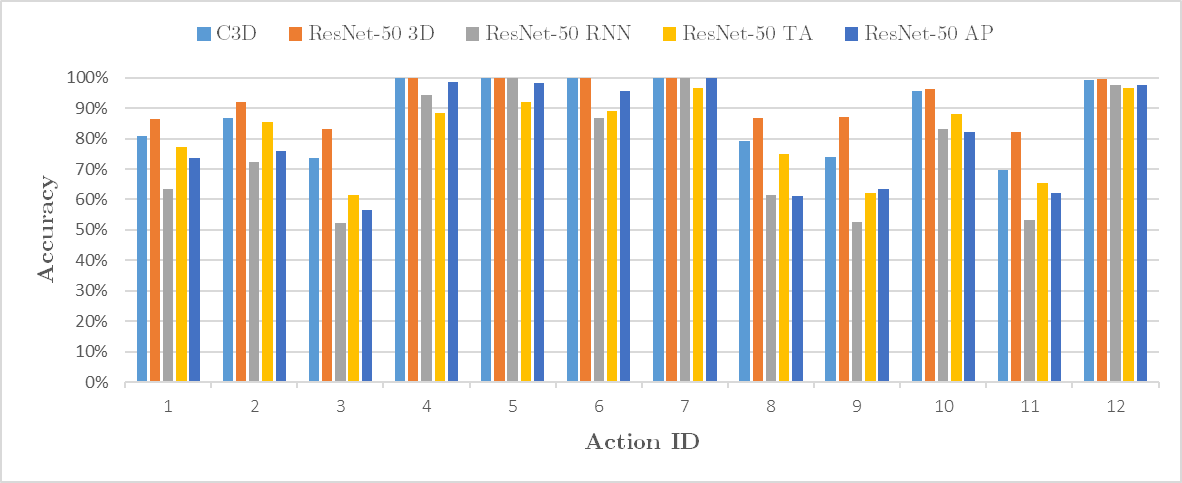
\includegraphics[width=0.8\linewidth]{figs/pc-MvDA_confusion_ixmas.png}
        \caption{Comparison of accuracy on each action class using different deep features combined with pc-MvDA on IXMAS dataset}
        %\vspace{-0.3cm}
        \label{fig:pc-MvDA_confusion_ixmas}
    \end{figure}

    Table.\ref{tab:sota_ixmas} compares our best combination of ResNet-50 3D and pc-MvDA with state-of-the-art frameworks. The comparison is for reference only because in other works, low-level hand-crafted video representation is used as private features and train-test strategy is leave-one-class out, which is not applicable to our supervised deep feature extractors. However, the results are still commensurable. % in circumstances where supervised approaches are adopted.
    % TODO - High priority

    \begin{table}[htbp]
    \centering
    \caption{Comparison of our proposed methods with SOTA methods on IXMAS dataset according to the second evaluation protocol}
    \resizebox{0.7\textwidth}{!}{
    \begin{tabular}{|c|c|c|}
    \hline
    Methods                                                              & Cross-view & Multi-view \\ \hline
    Liu et al. \cite{liu2011cross}                                   & 76.32      & N/A       \\ \hline
    Zheng et al. \cite{zheng2012cross}                               & 95.1       & 99.32     \\ \hline
    Zheng et al. \cite{zheng2016cross}                               & 97.8       & 99.4      \\ \hline
    Kong et al. \cite{kong2017deeply}                                & 99.92      & 100       \\ \hline
    Ulhaq et al. \cite{ulhaq2017space}                               & 66.82      & 92.47     \\ \hline
    Zhang et al. \cite{zhang2018cross}                               & 84.1       & N/A        \\ \hline
    Liu et al. \cite{liu2018learning}                                & N/A        & 90.3     \\ \hline
    Liu et al. \cite{liu2018hierarchically}                          & 99.95      & 99.67     \\ \hline
    Our proposed method (ResNet-50 3D + pc-MvDA)                     & 99.67      & 99.65       \\ \hline
    \end{tabular}}
    \label{tab:sota_ixmas}
    \end{table}
